% Setup document for double sided A4 paper
\documentclass[11pt,a4paper,twoside,openright]{report}
\usepackage[a4paper,left=3.5cm, right=2.5cm, top=3.5cm, bottom=3.5cm]{geometry}

% Setup image path
\usepackage{graphicx}
\graphicspath{{./images}}

\usepackage{ifthen}
\usepackage{amsmath}
\usepackage{pdfpages}

\usepackage{cmbright}                 % Setup font
\usepackage{listings}                 % For displaying of source code
\usepackage{hyperref}			            % To make PDF navigatable
\usepackage[small,bf,hang]{caption}   % To improve captions

\usepackage{style/fiiw}

\title{Low-energy communication backup system for hydrogen racecar}
\subtitle{}

\forenameA{Jarno}
\surnameA{Mechele}

\forenameB{Joey}
\surnameB{De Smet}

\forenameC{Robijn}
\surnameC{Ameye}

\opleiding{Industriële wetenschappen}
\afdeling{Elektronica-ICT}

\academicyear{2024--2025}
\campus{brugeseng}
\promotorA[Begeleider]{Sammy Verslype}
\promotorB[Begeleider]{Anton Lintermans}

\begin{document}
\titlep

\section{Firmware Design and Implementation}

This section describes the firmware developed for the STM32U5 microcontroller~\cite{stm32u5}, which forms the core of our low-energy backup communication system. It handles real-time LoRa communication, sensor data acquisistion, and voice output via speech synthesis or WAV playback. To guarantee deterministic timing, we bui9ld on FreeRTOS~\cite{freertos}, as illustraded in Figure~\ref{fig:firmware-system}. Task isolation and priority levels make the codebase modular and maintainable.

\begin{figure}[H]
\centering
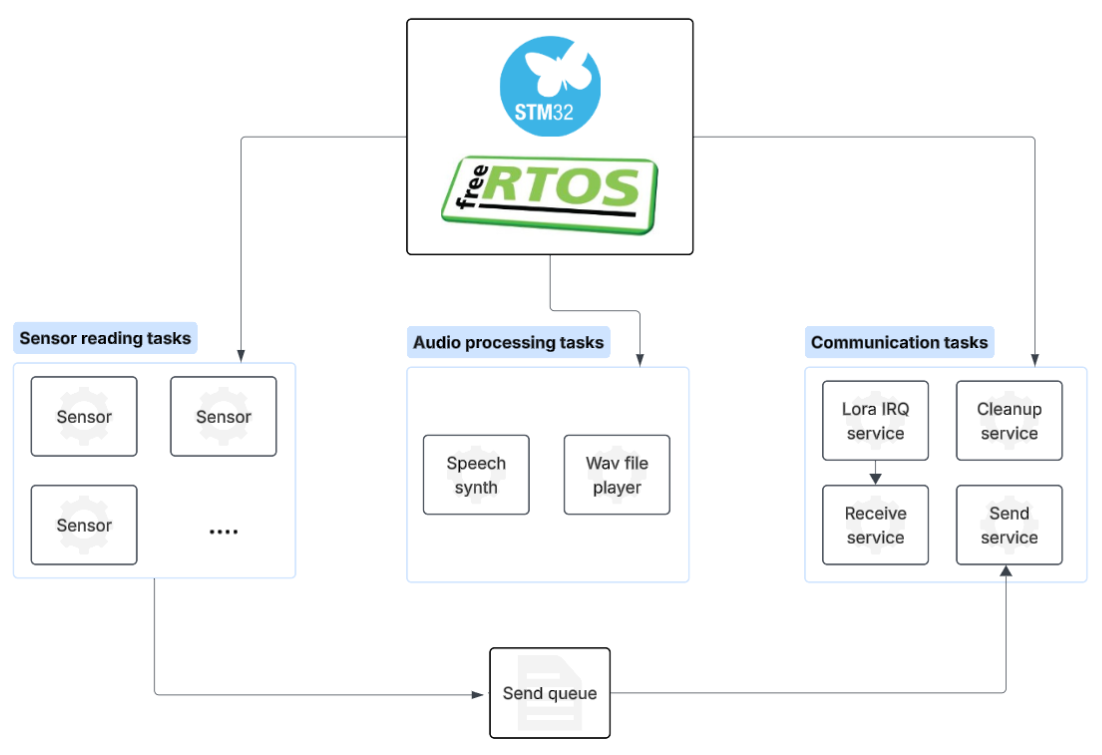
\includegraphics[width=0.45\textwidth]{images/firmware-system-design.png}
\caption{Overview of the FreeRTOS-based firmware architecture}\label{fig:firmware-system}
\end{figure}

\subsection{Overall Architecture}

Figure~\ref{fig:firmware-system} shows three primary functional domains, each implemented as one or more FreeRTOS tasks communicating via inter-task communication mechanisms provided by FreeRTOS.

\subsection{LoRa Communication}
\begin{itemize}
  \item \textbf{IRQ Handler}
    Waits on the SX1276~\cite{sx1276} interrupt line to detect packet RX/TX completion, then gives a binary semaphore.
  \item \textbf{Receive Task}
    Blocks on that semaphore, retrieves incoming packets, decrypts them with hardware-accelerated AES-128 in CTR mode, and forwards them for processing.  
  \item \textbf{Transmit Task}
    Pulls outgoing messages from a FreeRTOS queue, encrypts and formats them, then issues the LoRa send command.
  \item \textbf{Cleanup Task}
    Periodically scans stored packet buffers for timeouts and frees associated heap memory.
\end{itemize}

\subsection{Sensor Management}
Each sensor (e.g.\ temperature, pressure, speed) runs its own task at a low priority. Tasks periodically sample the hardware interface, package reacdings, and enqueues them for transmission.

\subsection{Audio Processign}
\begin{itemize}
  \item \textbf{Speech Synthesis Task}
    A port of \texttt{espeak-ng}~\cite{espeakng} with all file I/O replaced bu in-memory C arrays. Wich dequeues strings from a FreeRTOS queue, synthesises, streams audio to I2S hardware.
  \item \textbf{WAV playback Task}
    Streams hard-coded WAV data (e.g.\ racing flags, standard phrases) to the I2S hardware.
\end{itemize}

\subsection{Power and Memory Management}

All tasks are assigned carefully chosen priorities (Table~\ref{tab:priorities}) so that time-critical communication tasks preempt lower-priority work. We enable FreeRTOS tickless idle to allow the STM32U5 to enter deep sleep whenever the system is idle.

\begin{table}[H]
  \centering
  \caption{Task priorities and stack usage}
  \label{tab:priorities}
  \begin{tabular}{lrr}
    \hline
    Task                     & Priority & Stack (bytes) \\
    \hline
    LoRa IRQ Handler         & 8        & 128            \\
    Speech Synthesis         & 7        & 48\,000        \\
    WAV Playback             & 7        & 256            \\
    LoRa Transmit            & 5        & 128            \\
    Cleanup                  & 5        & 128            \\
    Sensor (each)            & 3        & 256            \\
    \hline
  \end{tabular}
\end{table}


\begin{picture}(0,0)(0,26)
  \hspace*{-10em}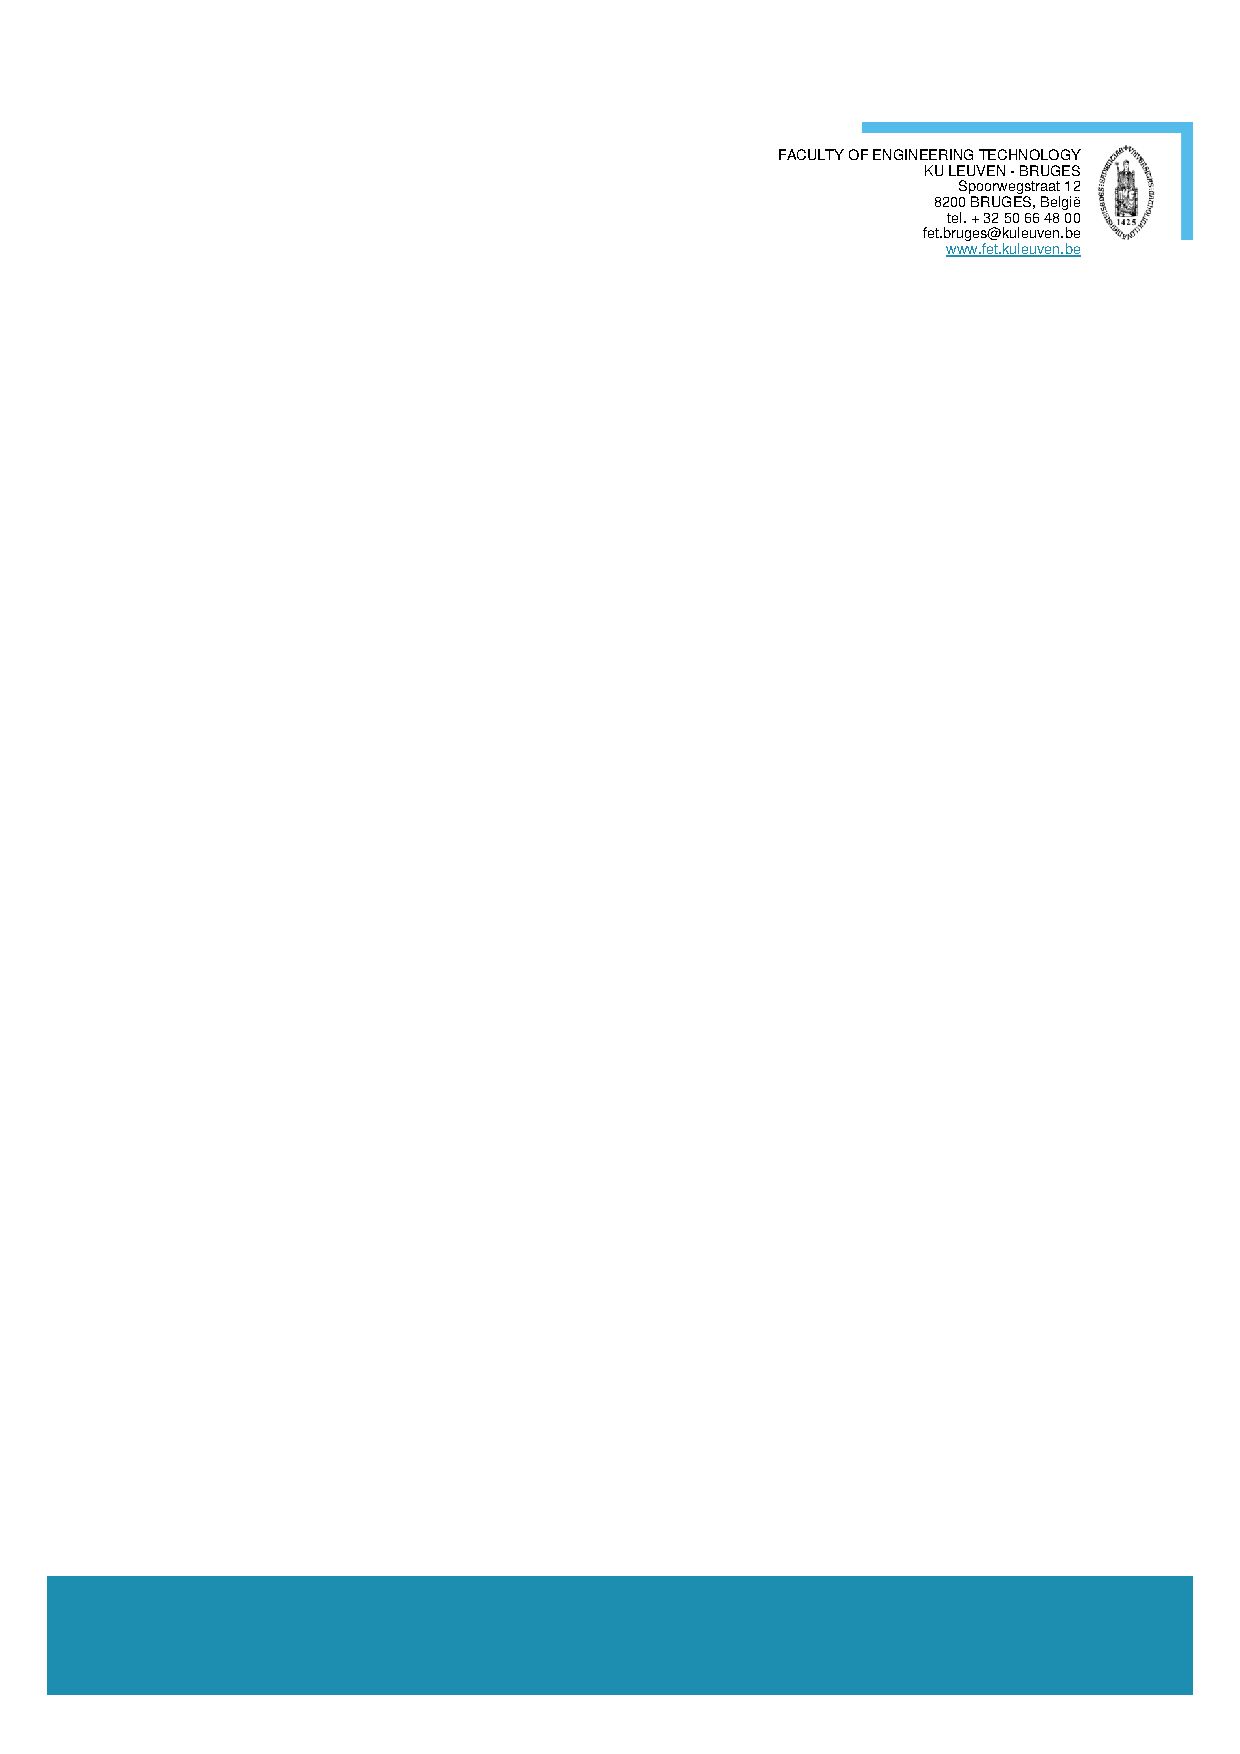
\includegraphics[width=\paperwidth]{covers/back_fiiw_bruges_eng.pdf}
\end{picture}%
\end{document}
